\documentclass[11pt,a4paper]{article}
\usepackage{graphicx} 
\usepackage{multirow}
\usepackage{enumitem}
\usepackage{amssymb}
\usepackage{amsmath}
\usepackage{amsthm}
\usepackage{xcolor}
\usepackage{tikz}
\usepackage{pgfplots}
\pgfplotsset{compat=1.18}
\usepackage{geometry}
	\geometry{
		total = {160mm, 237mm},
		left = 20mm,
		right = 35mm,
		top = 20mm,
		bottom = 20mm,
	}
\usepackage{hyperref}
\hypersetup{
    colorlinks=true,
    linkcolor=blue,
    filecolor=magenta,      
    urlcolor=cyan,
    pdftitle={Overleaf Example},
    pdfpagemode=FullScreen,
    }
\usepackage{fancyhdr}
\renewcommand{\headrulewidth}{0pt}
\renewcommand{\arraystretch}{1.1}
\pagestyle{fancy}

\graphicspath{{C:/Users/teoso/OneDrive/Documents/Tugas Kuliah/Template Math Depart/}}

\newcommand{\R}{\mathbb{R}}
\newcommand{\N}{\mathbb{N}}
\newcommand{\Z}{\mathbb{Z}}
\newcommand{\Q}{\mathbb{Q}}
\newcommand{\jawab}{\textbf{Solusi}:}

\newtheorem*{teorema}{Teorema}
\newtheorem*{definisi}{Definisi}

\begin{document}
\fancyfoot[C]{\raisebox{.5ex}{\rule{0.5cm}{.4pt}}o0o\raisebox{.5ex}{\rule{0.5cm}{.4pt}}}
\noindent
\begin{table}[h!]
  \centering
  \begin{tabular}{r c l}
    \includegraphics[width=2cm]{ITS.png}
     & \begin{tabular}{|c|l|l|}
         \hline
         \multirow{3}{*}{{\Huge \textbf{EAS}}}        & \textbf{Matakuliah}    & Geometri Analitik (A,B,C,D)         \\
         \cline{2-3}
                                                      & \textbf{Semester}      & 1                                   \\
         \cline{2-3}
         \multirow{3}{*}{{\large \textbf{GASAL}}}     & \textbf{Kredit SKS}    & 3                                   \\
         \cline{2-3}
         \multirow{3}{*}{{\large \textbf{2023/2024}}} & \textbf{Hari, Tanggal} & Jumat, 15 Desember 2023             \\
         \cline{2-3}
                                                      & \textbf{Waktu}         & \textbf{100 menit}                  \\
         \cline{2-3}
                                                      & \textbf{Dosen}         & \begin{tabular}{l}
                                                                                Drs. I Gst Ngr Rai Usadha, M.Si.   \\
                                                                                Dra, Wahyu Fistia Doctorina, M.Si. \\
                                                                                Drs. Komar Baihaqi, M.Si.          \\
                                                                                DR. Mont Kistosil Fahim, S.Si, M.Si.
                                                                              \end{tabular} \\
         \hline
       \end{tabular}
     &
    \includegraphics[width=2cm]{M.png}
    \\
  \end{tabular}
\end{table}
\begin{enumerate}
  \item Sketsa permukaan
        $
          x^2 - y^2 - z^2 = 16.
        $

  \item Dapatkan $z_x, z_y, z_{xx}, z_{yy}$, dan $z_{xy}$ dari
        $
          x^2 + y^2 - z^2 = 4.
        $

  \item Dapatkan hampiran persentase kesalahan maksimum untuk isi kerucut jika tingginya $30\,\text{cm}$ terjadi kesalahan pengukuran sebesar $1\%$ dan jari-jari lingkaran alasnya $10\,\text{cm}$ dengan kesalahan pengukuran sebesar $\tfrac{1}{2}\%$. Tentukan nilai hampiran ukuran minimum dan maksimum isi kerucut tersebut.

  \item Dapatkan persamaan bidang singgung dan garis normal terhadap permukaan
        $
          z + 1 = x e^{y} \cos z
        $
        di titik $(1, 0, 0)$.

  \item Kuadrat jarak titik asal ke permukaan $xyz = 1$ adalah
        $
          d^2 = x^2 + y^2 + z^2.
        $
        Dapatkan jarak terpendek dari titik asal ke permukaan $xyz = 1$ tersebut.
\end{enumerate}
\begin{center}
  \textbf{== HARAP JUNJUNG TINGGI KEJUJURAN ==}
\end{center}
\newpage
\fancyhead[L]{\textit{Solution By: \hyperlink{https://github.com/TetewHeroez}{Tetew}}}
\fancyfoot[C]{}
{\centering
  \textbf{SOLUSI}
  \par
}
\begin{enumerate}
  \item Andaikan kita tidak mengetahui bahwa itu adalah hiperboloid, kita bisa pandang persamaan diatas dalam 3 POV yaitu bidang $xy$, $xz$, dan $yz$.
        \begin{itemize}
          \item Pada bidang $xy$ (jika $z = 0$), maka diperoleh
                $
                  x^2 - y^2 = 16,
                $
                yaitu hiperbola terbuka ke arah sumbu $x$. Gambarnya seperti berikut.
                \begin{center}
                  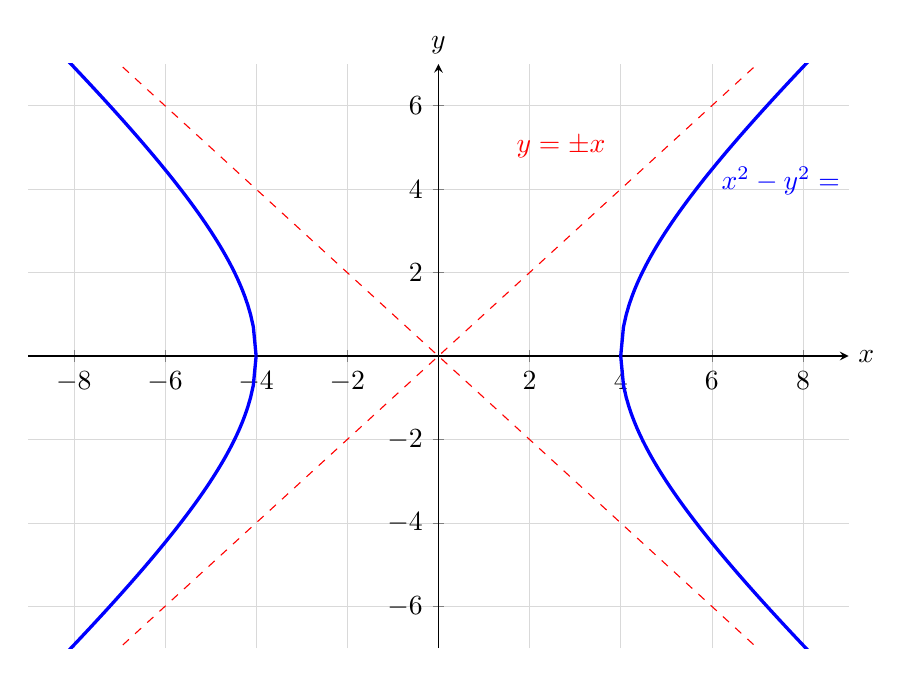
\begin{tikzpicture}
                    \begin{axis}[
                        axis lines=middle,
                        xlabel={$x$}, ylabel={$y$},
                        xlabel style={right},
                        ylabel style={above},
                        xmin=-9, xmax=9, ymin=-7, ymax=7,
                        xtick={-8,-6,-4,-2,0,2,4,6,8},
                        ytick={-6,-4,-2,0,2,4,6},
                        grid=both,
                        grid style={line width=.1pt, draw=gray!20},
                        major grid style={line width=.2pt,draw=gray!30},
                        samples=200,
                        domain=4:10,
                        restrict y to domain=-100:100,
                        width=12cm,height=9cm,
                        clip=true
                      ]

                      % Cabang kanan (y positif)
                      \addplot [very thick, blue, domain=4:10, samples=100] {sqrt(x^2 - 16)};
                      % Cabang kanan (y negatif)
                      \addplot [very thick, blue, domain=4:10, samples=100] {-sqrt(x^2 - 16)};
                      % Cabang kiri (y positive)
                      \addplot [very thick, blue, domain=-10:-4, samples=100] {sqrt(x^2 - 16)};
                      % Cabang kiri (y negative)
                      \addplot [very thick, blue, domain=-10:-4, samples=100] {-sqrt(x^2 - 16)};

                      % Asimtot y = x dan y = -x
                      \addplot [dashed, red, domain=-8:8] {x};
                      \addplot [dashed, red, domain=-8:8] {-x};

                      % Label hiperbola (opsional)
                      \node[blue,right] at (axis cs:6,4.2) {$x^2-y^2=16$};
                      \node[red,right] at (axis cs:1.5,5) {$y=\pm x$};
                    \end{axis}
                  \end{tikzpicture}
                \end{center}

          \item Pada bidang $xz$ (jika $y = 0$), maka diperoleh
                $
                  x^2 - z^2 = 16,
                $
                yaitu hiperbola terbuka ke arah sumbu $x$. Gambarnya seperti berikut.
                \begin{center}
                  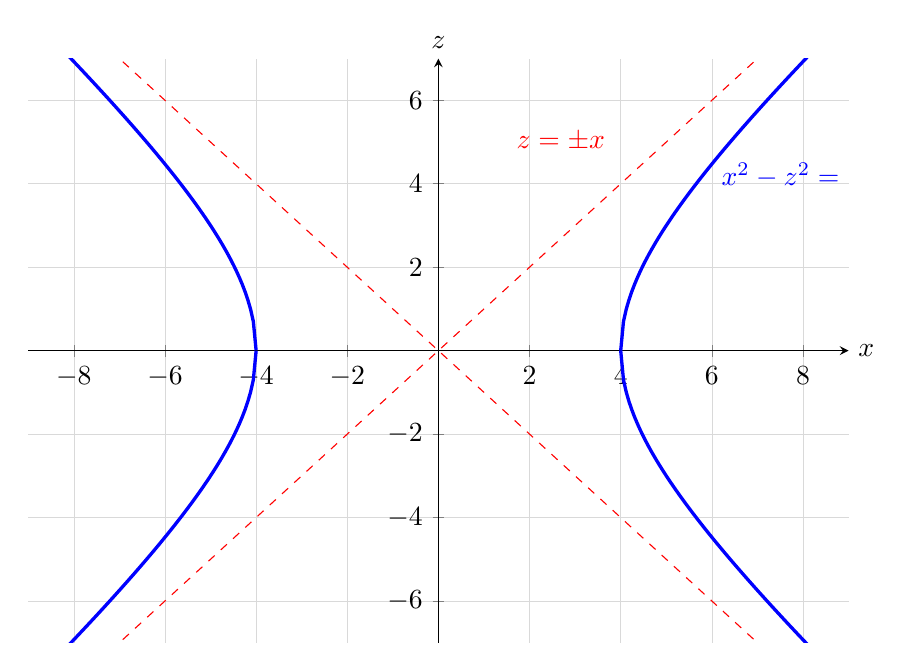
\begin{tikzpicture}
                    \begin{axis}[
                        axis lines=middle,
                        xlabel={$x$}, ylabel={$z$},
                        xlabel style={right},
                        ylabel style={above},
                        xmin=-9, xmax=9, ymin=-7, ymax=7,
                        xtick={-8,-6,-4,-2,0,2,4,6,8},
                        ytick={-6,-4,-2,0,2,4,6},
                        grid=both,
                        grid style={line width=.1pt, draw=gray!20},
                        major grid style={line width=.2pt,draw=gray!30},
                        samples=200,
                        domain=4:10,
                        restrict y to domain=-100:100,
                        width=12cm,height=9cm,
                        clip=true
                      ]

                      % Cabang kanan (z positif)
                      \addplot [very thick, blue, domain=4:10, samples=100] {sqrt(x^2 - 16)};
                      % Cabang kanan (z negatif)
                      \addplot [very thick, blue, domain=4:10, samples=100] {-sqrt(x^2 - 16)};
                      % Cabang kiri (z positive)
                      \addplot [very thick, blue, domain=-10:-4, samples=100] {sqrt(x^2 - 16)};
                      % Cabang kiri (z negative)
                      \addplot [very thick, blue, domain=-10:-4, samples=100] {-sqrt(x^2 - 16)};

                      % Asimtot z = x dan z = -x
                      \addplot [dashed, red, domain=-8:8] {x};
                      \addplot [dashed, red, domain=-8:8] {-x};

                      % Label hiperbola (opsional)
                      \node[blue,right] at (axis cs:6,4.2) {$x^2-z^2=16$};
                      \node[red,right] at (axis cs:1.5,5) {$z=\pm x$};
                    \end{axis}
                  \end{tikzpicture}
                \end{center}
          \item Pada bidang $yz$ (jika $x = 5$ atau $x = -5$), maka diperoleh
                $
                  -y^2 - z^2 = 16 - 25 = -9 \implies y^2 + z^2 = 9,
                $
                yaitu lingkaran dengan jari-jari $3$. Gambarnya seperti berikut.
                \begin{center}
                  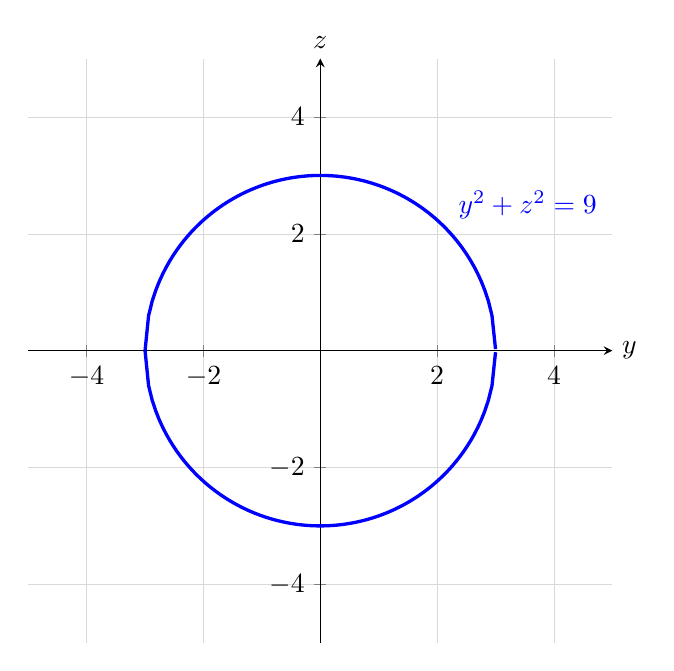
\begin{tikzpicture}
                    \begin{axis}[
                        axis lines=middle,
                        xlabel={$y$}, ylabel={$z$},
                        xlabel style={right},
                        ylabel style={above},
                        xmin=-5, xmax=5, ymin=-5, ymax=5,
                        xtick={-4,-2,0,2,4},
                        ytick={-4,-2,0,2,4},
                        grid=both,
                        grid style={line width=.1pt, draw=gray!20},
                        major grid style={line width=.2pt,draw=gray!30},
                        samples=200,
                        domain=-3:3,
                        restrict y to domain=-100:100,
                        width=9cm,height=9cm,
                        clip=true
                      ]

                      % Lingkaran y^2 + z^2 = 9
                      \addplot [very thick, blue, domain=-3:3, samples=100] {sqrt(9 - x^2)};
                      \addplot [very thick, blue, domain=-3:3, samples=100] {-sqrt(9 - x^2)};

                      % Label lingkaran (opsional)
                      \node[blue,right] at (axis cs:2.2,2.5) {$y^2+z^2=9$};
                    \end{axis}
                  \end{tikzpicture}
                \end{center}
        \end{itemize}
        Kemudian jika kita gabungkan ketiga gambar diatas dalam bentuk 3D, maka kita akan mendapatkan gambar berikut.
        \begin{center}
          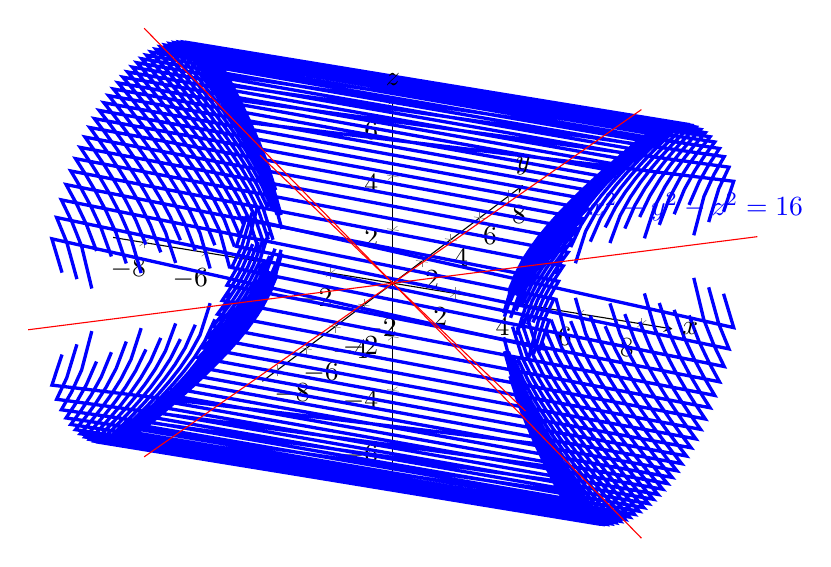
\begin{tikzpicture}
            \begin{axis}[
                axis lines=center,
                xlabel={$x$}, ylabel={$y$}, zlabel={$z$},
                xlabel style={right},
                ylabel style={above},
                zlabel style={above},
                xmin=-9, xmax=9, ymin=-9, ymax=9, zmin=-7, zmax=7,
                xtick={-8,-6,-4,-2,0,2,4,6,8},
                ytick={-8,-6,-4,-2,0,2,4,6,8},
                ztick={-6,-4,-2,0,2,4,6},
                grid=both,
                grid style={line width=.1pt, draw=gray!20},
                major grid style={line width=.2pt,draw=gray!30},
                samples=50,
                domain=-8:8,
                restrict y to domain=-100:100,
                width=12cm,height=10cm,
                clip=true
              ]

              % Permukaan hiperboloid
              \addplot3 [very thick, blue, domain=-8:8, y domain=-8:8] ({x}, {y}, {sqrt(x^2 - y^2 - 16)});
              \addplot3 [very thick, blue, domain=-8:8, y domain=-8:8] ({x}, {y}, {-sqrt(x^2 - y^2 - 16)});

              % Asimtot pada bidang xy
              \addplot3 [dashed, red, domain=-8:8] ({x}, {x}, {0});
              \addplot3 [dashed, red, domain=-8:8] ({x}, {-x}, {0});

              % Asimtot pada bidang xz
              \addplot3 [dashed, red, domain=-8:8] ({x}, {0}, {x});
              \addplot3 [dashed, red, domain=-8:8] ({x}, {0}, {-x});

              % Label permukaan (opsional)
              \node[blue,right] at (axis cs:6,0,4) {$x^2-y^2-z^2=16$};
            \end{axis}
          \end{tikzpicture}
        \end{center}

\end{enumerate}
\end{document}